% !TeX root = ../praktikum.tex
% !TeX encoding = UTF-8
% !Tex spellcheck = de_DE

In diesem Versuchsabschnitt werden die beiden zu untersuchenden Effekte gemessen, während an der Probe ein Gleichstrom anliegt. Hierzu wird gleichzeitig der Spannungsabfall über die Länge und über die Breite der Probe mit der Software erfasst. An die Probe wird in x-Richtung ein konstanter Gleichstrom von $\unit[1]{\mu A}$ angelegt. Um eine stabile Temperatur zu erhalten, wurde die Kammer auf \unit[2]{K} geheizt. Jetzt wurde das Magnetfeld auf \unit[-7]{T} gefahren. Dies dauert rund sieben Minuten, da es sich um supraleitende Spulen handelt und das Anlegen eines Stroms eine Gegeninduktion verursacht. Sobald das Magnetfeld aufgebaut ist, wird die Hallspannung $U_H$ sowie die Längsspannung $U_{xx}$ aufgezeichnet, während das Magnetfeld mit etwa \unitfrac[1]{T}{min} auf \unit[7]{T} gefahren wird. 


Diese Messdaten sind zusammen mit einer weiteren Messung im Bereich von $-2$ bis \unit[+2]{T} bei einer konstanten Erhöhung von \unitfrac[0,2]{T}{min} in Abbildung~\ref{fig:full_range_dc} aufgetragen.

\begin{figure}[h]
	\centering
	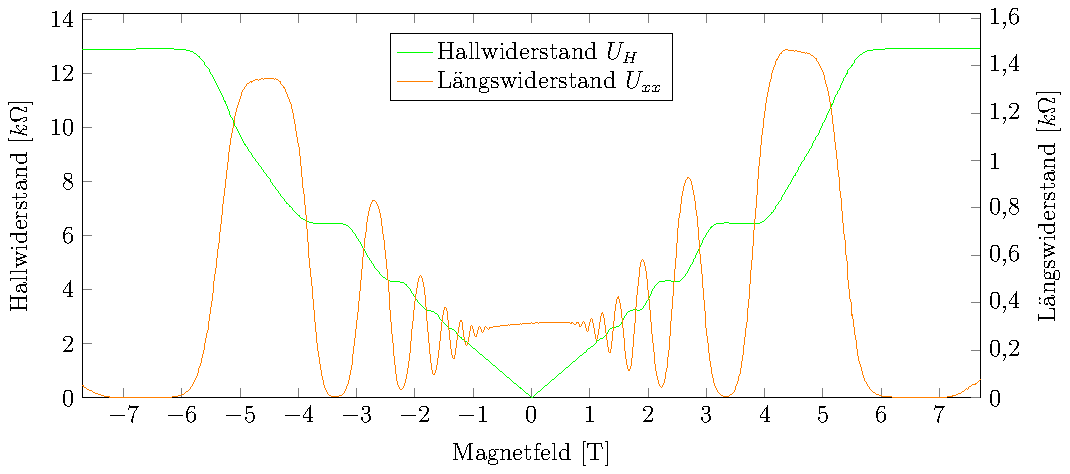
\includegraphics{graphs/dc/full_range.pdf}
	\caption[Gleichstrommessung im maximalen Magnetfeldbereich]{
		Hall-Widerstand und Shubnikov-de Haas Oszillationen eines mit Gleichstrom durchflossenen 2DES.
	}
	\label{fig:full_range_dc}
\end{figure}

Es sind deutlich die Plateaus des Hall- und Shubnikov-de Haas-Widerstandes zu erkennen.


\begin{figure}[h]
	\centering
	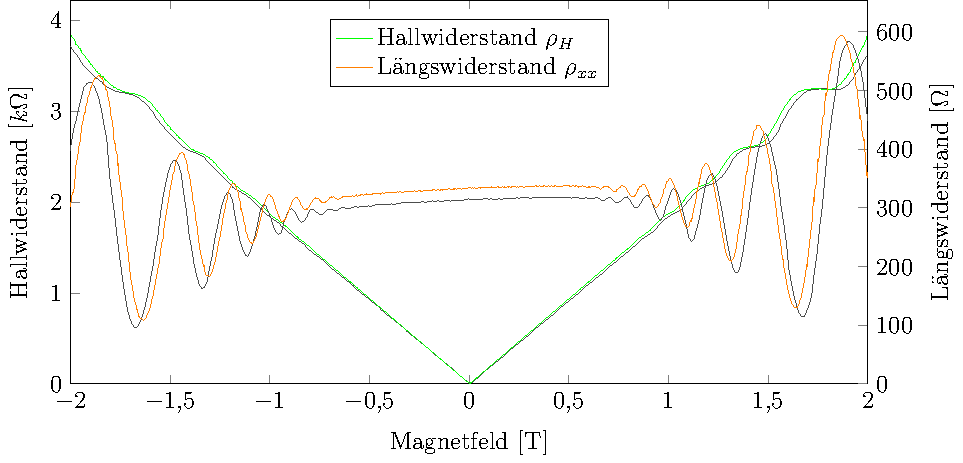
\includegraphics{graphs/dc/pm2T_range.pdf}
	\caption[Höher aufgelöste Gleichstrommessung in Magnetfeldteilbereich]{
		Hall-Widerstand und Shubnikov-de Haas Oszillationen eines mit Gleichstrom durchflossenen 2DES.
	}
	\label{fig:2T_range_dc}
\end{figure}